
\subsection{Bias Variance Trade-off}

\begin{frame}
    \frametitle{Bias Variance Trade-off}
    \framesubtitle{The Expected Generalization Error}
    \onslide<1->{
        \begin{center}
            $y = f(x) + \epsilon$ \\
            $\epsilon \sim \mathcal{N}(0,\sigma_{\epsilon}^2)$
            $D = \{(x_{1},y_{1}), (x_{2}, y_{2}), ... , (x_{N}, y_{N})\}$
        \end{center}
    }
    \onslide<2->{
        The decomposition of a model's expected generalization error is
        \begin{align*}
            \boldsymbol{Err}(\hat{f}(x)) = \sigma_{\epsilon}^2 + [Bias(\hat{f}(x))]^2 + Var(\hat{f}(x))
        \end{align*}
    }
    \onslide<3->{
        $\sigma_{\epsilon}^2$ is irreducible and independent of the model. \\
        \bigskip
        Trade-off between bias and variance. \\
        \textbf{Aim:} Adjusting parameters to decrease variance keeping bias unaffected.
        }
\end{frame}

\begin{frame}
    \frametitle{Bias-Variance Trade-off}
    \framesubtitle{Illustration}
    \onslide<1->
        \begin{figure}      
            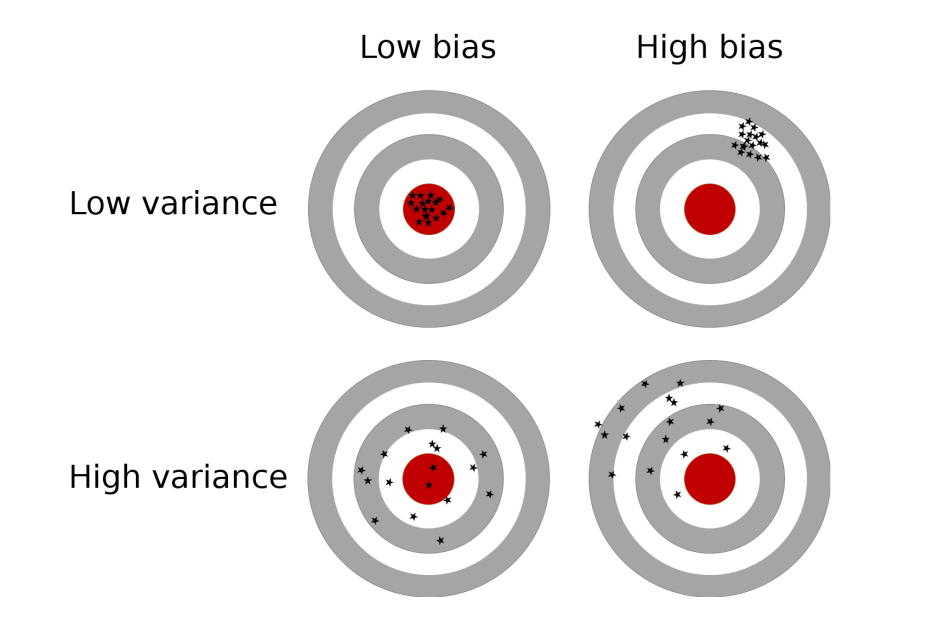
\includegraphics[height=0.6\textheight]{images/bias-variance.png}
            \caption{Illustration of bias-variance trade-off \cite{van2019bias}}
        \end{figure}
    \onslide<2->{
        \begin{center}
        Decision trees generally have low bias and high variance \cite{friedman2001elements}.
        \end{center}
    }
\end{frame}

    %\begin{columns}[c] % The "c" option specifies centered vertical alignment while the "t" option is used for top vertical alignment
    
    %\column{.45\textwidth} % Left column and width
    %\textbf{Heading}
    %\begin{enumerate}
    %\item Statement
    %\item Explanation
    %\item Example
    %\end{enumerate}
    
    %\column{.5\textwidth} % Right column and width
    %Lorem ipsum dolor sit amet, consectetur adipiscing elit. Integer lectus nisl, ultricies in feugiat rutrum, porttitor sit amet augue. Aliquam ut tortor mauris. Sed volutpat ante purus, quis accumsan dolor.
    
    %\end{columns}
